\chapter{实验与评估} \label{experiment}

进行的实验主要有两部分,真机的SLAM实验和地图融合实验。

\section{真机配置与实验}

真机使用单机实验。

真机搭载英特尔T265摄像头,其特点是带两个鱼眼镜头和惯性测量单元,并且视觉SLAM可以运行在其特有的视觉处理单元上。其在电脑上需要一定配置,安装英特尔的一些以来库文件和realsense-viewer。

除摄像头外,真机还搭载Jetson Xavier NX计算机,体积较小且接口丰富。需要注意的是,无人机在地面时,可以使用显示器和鼠标设备对其进行操作,运行ROS节点;但当无人机在空中时,没有显示信息和鼠标的操作输入,因此需要使用远程控制,在这里使用了No Machine软件进行远程控制。

实验内容;



\section{地图融合实验}

在教学楼楼道场景下,使用手持相机的方式,沿楼道行走,完成对一段楼道的建图;同时准备另一台相机,沿不同的路线行进,完成对同一段楼道的建图;两段视频应该拥有一部分重合的场景和一部分不重合的场景,用以验证地图融合的效果。

需要注意的是,使用单目视觉SLAM时,初始化是一个重要的步骤,一般采用在一个场景左右平移的方法完成初始化,之后才能进行跟踪进程,否则一段视频中将会有大量的时间用于初始化,这也意味着选取视频的质量十分重要。

在进行SLAM进程前,需要对相机进行标定,可以采用张正友标定法;需要注意的是,相机的拍照模式和录像模式,其内参矩阵可能不同;对于使用视觉SLAM的相机,建议采用动态标定法。

最后,使用预先录制的视频验证SLAM算法有两个方式:

\begin{enumerate}
	\item 将视频转换成KITTI或TUM数据集的格式;通过观察这些数据集的格式可以看出,其一般是灰度图加深度信息,并且配有时间戳,这样的转换可能有一些复杂。转换完成后,使用ROS的例子中自带的对于特定传感器和特定数据集的可执行文件运行整个SLAM进程即可。
	\item 较为简单的方式是将其转换为ROS的rosbag,rosbag可以记录特定话题的信息;对于视频而言,即记录不同时间戳下矩阵各点的三通道RGB值,对于灰度视频则更为方便;其用法是使用ROS的cv bridge完成一些MP4格式视频到rosbag包的转换。
\end{enumerate}

完成MP4格式到rosbag的部分代码如下:

\begin{lstlisting}[language={C++}]
// set wait key = 1000/fps
cv::waitKey(int(1000/fps));

std_msgs::Header header;
header.frame_id = "frame";
header.stamp = ros::Time::now();

sensor_msgs::ImagePtr ImageMsg = cv_bridge::CvImage(header, "bgr8", frame).toImageMsg();

if(FrameNum % 2 == 0){
my_bag.write(topicName, ros::Time::now(), ImageMsg);
cout << "recording frames:" << frameNum << endl;
}
\end{lstlisting}

其主要逻辑是,将每一帧的信息转换成sensor\_msg类型的消息,之后写入到rosbag中。这里需要注意waitKey函数,其含义为循环等待,单位是1/1000秒,因此1000/fps即为按照fps帧率,每一帧需要等待的时间;该参数控制了视频的帧率,从而控制了rosbag包的长度。topicName为录制的话题名,已经提前定义好。

准备就绪后,进入SLAM程序,得到的结果如下:

\begin{figure}[!ht]
	\centering
	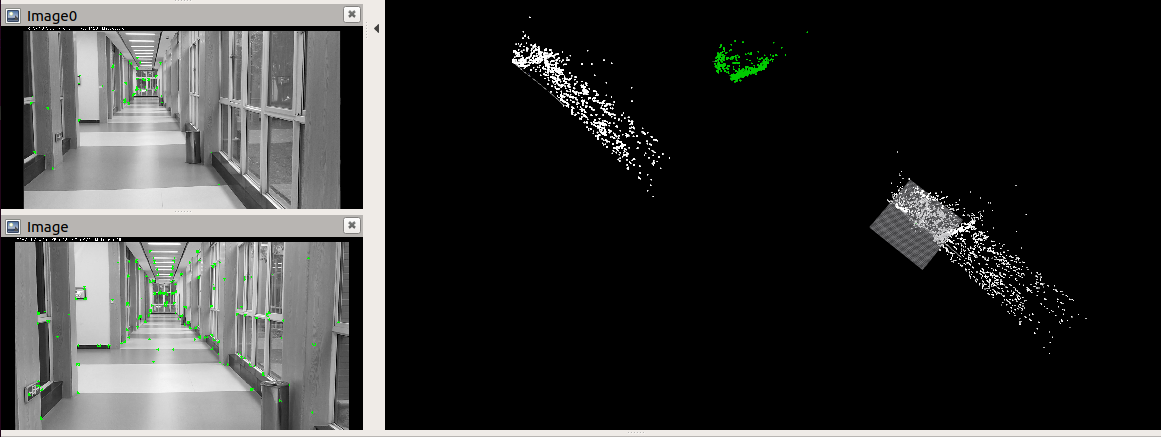
\includegraphics[width=0.9\textwidth]{ccm1.png}
	\caption{地图融合结果}
	\label{fig5-1}
\end{figure}

可以看出,基本完成了建图和地图融合的任务。